\capitulo{4}{Técnicas y herramientas}

Esta parte de la memoria tiene como objetivo presentar las técnicas metodológicas, bibliotecas, lenguajes y las herramientas de desarrollo que se han utilizado para llevar a cabo el proyecto. Se comentarán los aspectos más destacados de cada opción y se han añadido referencias bibliográficas que incluyen más información.

\section{Herramientas de metodología ágil}
\textbf{Git}

Git es un software de control de versiones (free and open source) diseñado por Linux Torvalds, centrado en la eficiencia, confiabilidad y compatibilidad del mantenimiento de versiones de aplicaciones con una gran cantidad de archivos de código fuente. 

La característica diferencial con el resto de SCM\footnote{\textbf{Gestión de configuración de Software} (Software Configuration Management, SCM) es una especialización de la gestión de la configuración de todas las actividades en el sector de desarrollo de software. SCM trata y controla: La elaboración de código fuente por varios desarrolladores simultáneamente} es su modelo de ramificación, permitiendo trabajar en ramas locales, para después poder realizar operaciones de fusión y eliminación del código con facilidad.

%\imagen{git_branches}{Ramificación git} 

Para más información: \url{https://git-scm.com/}

\textbf{GitHub} 

Github es una plataforma destinada a alojar proyectos para el control de versiones Git y desarrollo colaborativo software. 

Hemos utilizado GitHub debido a su facilidad de cara a trabajar con la metodología SCRUM, permitiéndonos dividir el proceso de desarrollo en períodos de trabajo o "sprints", y realizar análisis posteriores que nos mostrarán posibles errores de planificación y aciertos en cuanto al desarrollo del proyecto. Otro factor es su facilidad de interacción con otras herramientas.

Repositorio del proyecto en GitHub: \url{https://github.com/humbertoms99/DIET_COMPOSITION}

\textbf{ZenHub}

Para realizar el seguimiento de los desarrollo del proyecto se ha utilizado ZenHub, que es un extensión de Chrome que se integra de forma nativa en la interfaz de usuario de GitHub, y nos  ofrece un seguimiento de los requerimientos de nuestros repositorios. Nos permite realizar planificaciones junto con un seguimiento y posterior análisis. También incluye filtrado por etiquetas, agrupación de problemas, visualizar posibles bloqueadores, entre otras opciones. 

Conviene destacar la facilidad con se crean los gráficos de ejecución, seguimiento de la velocidad e informes de versión. Estos se  analizarán en los anexos de este proyecto.

Para más información: \url{https://www.zenhub.com/}

\section{Lenguajes de programación}


\textbf{HTML}

Es un lenguaje de marcado de hipertexto dedicado a la elaboración de código utilizado para estructurar y desplegar  páginas web.
HTML se escribe en forma de etiquetas rodeadas por corchetes angulares (<,>,/). Hemos utilizado este lenguaje en el proyecto de front-end  para realizar las vistas de nuestra web.

\textbf{Typescript}

Es un lenguaje fuertemente tipado basado en JavaScript. Se diferencia respecto a JavaScript en que añade tipos estáticos y objetos basados en clases.

\textbf{PHP}

Es un lenguaje de código abierto adecuado para desarrollo web y que puede ser incrustado en HTML. Lo que distingue a PHP es que el código se ejecuta en el servidor, al contrario que en lenguajes como Javascript, que se ejecutan del lado del cliente.

Para más información: \url{https://www.php.net/manual/es/}

\textbf{CSS}

Es un lenguaje de diseño gráfico o lenguaje de estilos para definir la presentación de un documento estructurado escrito en lenguajes de marcados (HTML o XML). Es uno de los lenguajes base para Webs; con él podemos alterar la fuente, color, tamaño y espaciado del contenido.

\textbf{JSON}

Es un formato de texto utilizado en el intercambio de datos. Se trata de un subconjunto de notación de objetos de JavaScript.
Este tipo de formato es el esperado al hacer peticiones a la API desde nuestro front en Angular, permitiendo enviar estructuras de datos que pueden ser leídas con facilidad.

\section{Patrones de diseño}

\textbf{MVC}

MVC (Modelo-Vista-Controlador) es un patrón de diseño de software utilizado para implementar interfaces de usuario, datos y lógica de control. Su característica  principal es la separación de código en tres partes:
\begin{enumerate}
	\item Modelo: contiene la representación de los datos y lógica de negocio.
	\item Vista:  diseño de la interfaz gráfica de usuario; contiene la información que se envía al cliente.
	\item Controlador: Actúa como intermediario entre Modelo y Vista, gestionando y transformando los datos.
\end{enumerate}

En el caso particular del desarrollo web, el modelo suele corresponder al propio \emph{"model"} de una tabla de base de datos, el  código suele estar escrito en Javascript, y la vista  en HTML / CSS.

\section{Frameworks y servicios}

\textbf{Visual Studio Code}

Es un editor de código fuente  que se ejecuta en Windows, macOS y Linux. Incluye soporte  para la depuración control integrado de Git. Algunas características que ofrece el framework:

1. IntelliSense, que es un conjunto de funcionalidades de edición de código como sugerencias  de métodos y propiedades de objeto, información de parámetros y sus tipos.

2. Depuración directa desde el editor. Visual Studio Code ofrece depuración de código con puntos de  interrupción, pilas de llamadas y una consola interactiva.

3. Comandos git incorporados, permitiendo realizar revisiones en el propio framework, pudiendo descartar cualquier servicio SCM alojado.
% [TODO NOTA A PIE Supply Chain Management]

4.  Una gran cantidad de extensiones que facilitan el rápido desarrollo y visualización del código.

5. Implementación y posibilidad de alojar sitos en React, Angular, Vue, Node, Python entre otros, además de almacenar y consultar datos relacionados.

Para más información: \url{https://code.visualstudio.com}

\textbf{Postman}

Postman es una plataforma de API que permite a los  desarrolladores testear sus APIs. Nos ofrece la posibilidad de simular peticiones HTTP request a través de una interfaz gráfica adaptada al usuario, por la cual podremos observar el estado de la respuesta y de los datos que se obtienen, posibles mensajes de validaciones. 

\begin{figure}[h!] 
\centering
    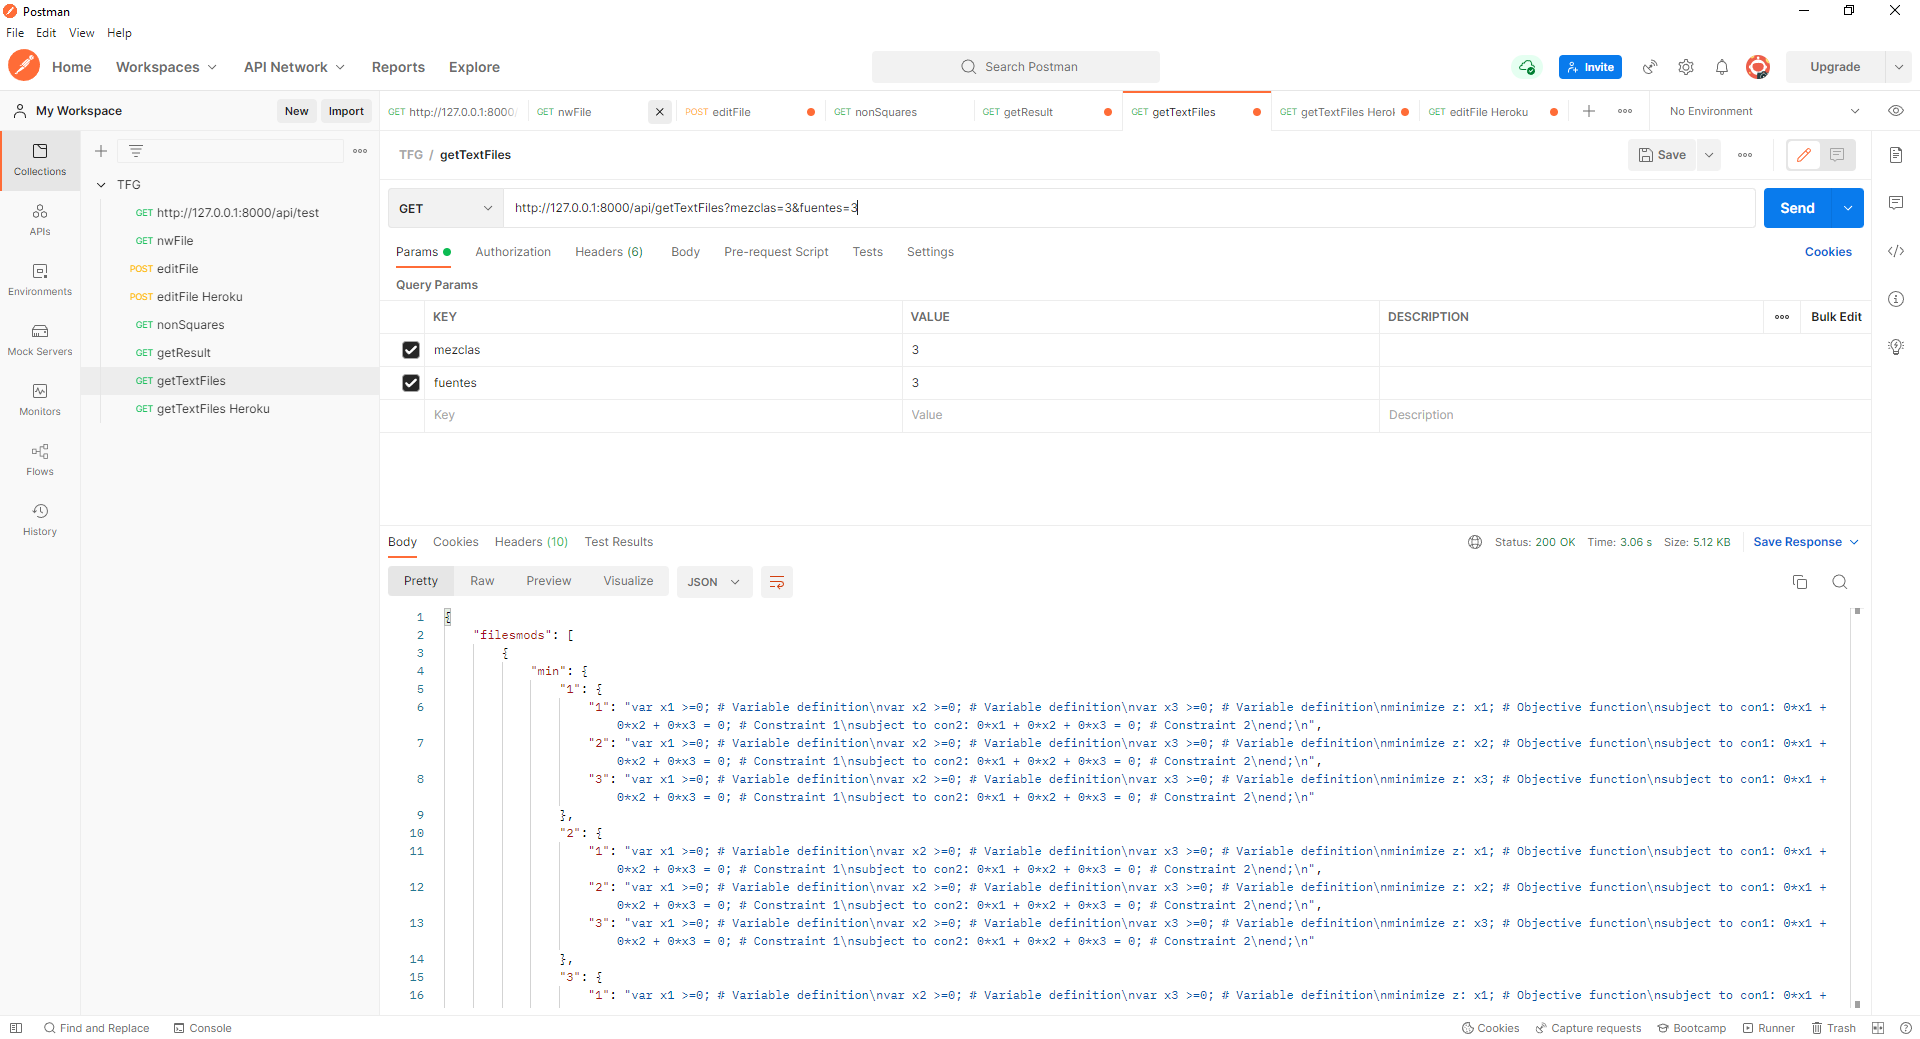
\includegraphics[width=1\textwidth]{img/postmanRequest.PNG}
\caption{Petición Postman}
\label{fig:request_postman}
\end{figure}

En la Figura \ref{fig:request_postman} se puede observar la interfaz de Postman, en la cual podemos organizar nuestras peticiones en Colecciones; a la derecha encontramos la url a la que se realiza la petición y el tipo operación. En la parte central nos permite introducir parámetros (hemos comprobado que ofrece la opción de introducir textos JSON  como parámetros). También nos ofrece la opción de configurar los headers y pasar un token en caso de nuestra API trabaje con un login previo.

Al lanzar la petición, retorna la repuesta en la parte inferior de la interfaz. En la esquina superior derecha se encuentra el status , es decir, si se ha realizado correctamente o si ha  llegado a un estado fallido (status 200: OK, status 4XX: Error en la petición al cliente, status 5XX: Error en el servidor).

El \textit{body} de la respuesta puede ser consultado en los siguientes formatos de texto: JSON, XML, HTML, Text o Auto, según nuestra elección.

Para más información: \url{https://www.postman.com/}

\textbf{Debian}

Debian es un sistema operativo libre desarrollado por la comunidad a través de la colaboración voluntaria. Hemos utilizado este subsistema a modo de terminal Linux para poder instalar la librería GLPK. Hemos seleccionado este sistema debido a compatibilidad  y facilidad de instalación desde Windows, que es el sistema operativo donde se han realizado los desarrollos del proyecto.

Para más información: \url{https://rincondelatecnologia.com/subsistema-linux-en-windows-10-que-es-para-que-sirve-y-como-instalarlo/}

%TODO: alternativas ubuntu otras terminales linux

\textbf{Angular}

Angular es un framework de JavaScript de código abierto, mantenido por Google, que se utiliza para  crear aplicaciones web \textit{Single Page Application}. Angular trabaja con el patrón de diseño MVC al ofrecer una separación clara entre las vistas y las funciones que realizan las operaciones con los datos, separando el lado del cliente del lado servidor. 

Angular está formado por un conjunto de herramientas para la interfaz de nuestra aplicación web; destaca su capacidad de adaptación permitiendo modificar sus características según el flujo de trabajo lo requiera, además de tener facilidad para incorporar otras librerías

Para más información: \url{https://www.udemy.com/course/angular-fernando-herrera}

\textbf{Angular Translate}

Angular translate es un modulo de Angular, que nos ha permitido internacionalizar la web a través de traducciones dinámicas. Su funcionamiento es por medio del pipe \textit{translate}, que busca el texto introducido en la carpeta \textit{i18n/**.json} y muestra su traducción correspondiente. En la figura \ref{fig:angular_translate} se realiza una traducción de la línea $26$ al inglés, añadiendo el pipe \textbf{translate} e incorporando el texto en el archivo de traducciones \textit{en.json} (Línea 3).

\begin{figure}[h!] 
\centering
    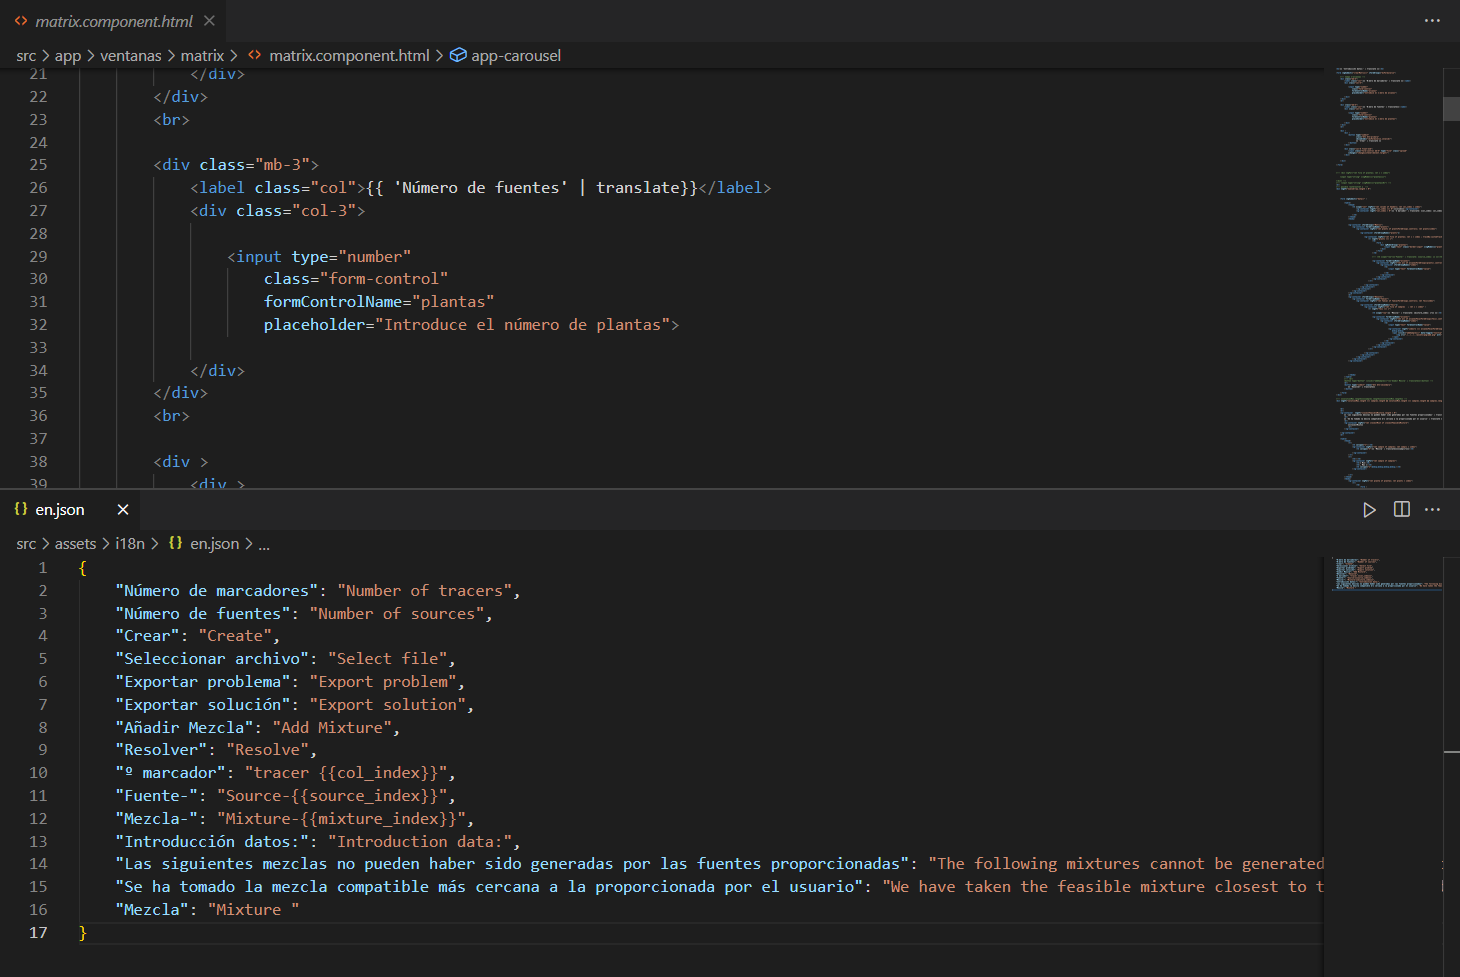
\includegraphics[width=0.8\textwidth]{img/translate.PNG}
\caption{Ejemplo Angular Translate}
\label{fig:angular_translate}
\end{figure}

\textbf{Angular Material}

Angular Material es un modulo de Angular, este modulo ofrece una biblioteca de componentes de interfaz de usuario (UI), los desarrolladores añaden estos componentes al modulo de Angular Material que a su vez es utilizado por el proyecto. Estos componentes nos  ofrecen interfaces de usuarios elegantes  y reutilizables, algunos componentes pueden ser botones, select, checkbox, table, Dialog, entre otros muchos.

Para trabajar con los componentes ofrecidos se ha seguido su documentación: \url{https://material.angular.io/components/categories}

\textbf{Bootstrap}

Bootstrap es una biblioteca multiplataforma o conjunto de herramientas de código abierto  para diseño de sitios y aplicaciones web. Incluye diseños plantilla para componentes habituales de las web, al igual que Angular Material. Una de sus características es su diseño adaptativo (\textit{"Responsive Design"}), que consiste en adaptar el diseño  de la aplicación a los distintos tamaños  de pantallas, permitiendo así acondicionar nuestras interfaces a los posibles cambios en el tamaño de pantalla.

Además ofrece la posibilidad de incluir esta librería por via CDN, que consiste en añadir un link en el archivo \textit{index.html} y carga automáticamente los estilos de bootstrap en la aplicación.


\textbf{Node.js}

Node.js es un entorno de ejecución para JavaScript construido con V8, basado en el motor de JavaScript de Chrome, con E/S de datos en una arquitectura orientada a eventos, y que utiliza un único hilo de ejecución asíncrono.

Para más información \url{https://nodejs.org/es/}

\textbf{npm}

Npm es un sistema de gestión de paquetes por defecto para Node.js. Coloca los módulos en su lugar para que Node pueda encontrarlos y gestionar los conflictos eficientemente.

Npm es muy configurable algunas de sus funcionalidades más comunes son la publicación, búsqueda, instalación y desarrollo de programas  node.

Con vista a la instalación de librerias, npm tiene dos modos: 
\begin{itemize}
	\item modo  global: npm instala los paquetes en \textit{prefix/lib/node\_modules} y los bins en \textit{prefix/bin}.
	\item modo local: npm instala los paquetes en el directorio del proyecto actual. Los paquetes en la ruta \textit{./node\_modules}, y los bins en ./bin.
\end{itemize}

\textbf{Heroku}

Heroku es una plataforma como  (PaaS) de computación en la Nube que soporta distintos lenguajes de programación. Heroku es propiedad de Salesforce.com. y ofrece servicios gratuitos para el despliegue proyectos.

Se ha utilizado para realizar el despliegue del back-end escrito en php en un servidor. 

\textbf{Netlify}

Netlify es una empresa  informática en la nube con sede en San Francisco que ofrece alojamiento a servicios para aplicaciones web y sitios estáticos.

En nuestro caso hemos hecho uso del paquete Starter gratuito para uso individual, y hemos desplegado el front-end en Angular, que llama a la API. .

\section{Librerias}

\textbf{glpk-5.0}

GLPK (GNU Linear Programming Kit) es un paquete destinado a resolver problemas de programación lineal, programación de enteros mixtos y otros problemas relacionados. Es un conjunto de rutinas  escritas en ANSI C y organizadas en forma de biblioteca invocable.

Se ha usado esta  librería en el back-end para resolver problemas de programación  linear mediante comandos que se ejecutan en una terminal Linux y tienen como resultado la generación de archivos .mod. Posteriormente veremos el análisis de estos archivos y datos requeridos para realizar el cálculo.

Para más información: \url{https://www.gnu.org/software/glpk/}

\textbf{libtsnnls-2.3.4}

Libtsnnls es un paquete de node que resuelve el problema de Fast Combinatorial Non-negative Least Squares. Se ha realizado la instalación con su comando  de instalación npm \textit{"npm i ml-fcnnls"} en el proyecto front y se ha usado para calcular las proyecciones de los puntos en el cono formado por las fuentes.

Para más información: \url{https://www.npmjs.com/package/ml-fcnnls/v/1.0.0}


\section{Otras Herramientas}

\textbf{Latex: TexStudio}

TexStudio es un editor de Latex de código abierto y Multiplataforma con una interfaz similar a Texmaker, que proporciona un soporte moderno de escritura, ofrece corrección ortográfica, plegado de código y resaltado de sintaxis. Ha aportado una revisión de la sintaxis de los documentos escritos en Latex.

Para más información: \url{https://www.texstudio.org/}


\textbf{Mendeley}

Mendeley es un gestor de referencias que se utiliza para administrar y compartir trabajos de investigación y la generación de bibliografías para artículos académicos. Se ha utilizado su aplicación de escritorio  \textit{Mendeley Reference Manager}.

Para más información: \url{https://www.mendeley.com/?interaction_required=true}


\textbf{Draw.io}

Draw.io es un software de dibujo gráfico  multiplataforma  gratuito y de código abierto desarrollado en HTML5 y JavaScript. Su interfaz permite crear diagramas de flujo, wireframes, diagramas UML, organigramas y diagramas de red. Se ha trabajo desde su versión online, y se ha elegido como  herramienta debido a su facilidad de uso y la cantidad de opciones de diseño que ofrece.

\textbf{Overleaf}

Overleaf es un  editor de textos Latex online que se utiliza para publicar documentos científicos, Se ha usado para realizar la documentación de este proyecto. Algunas ventajas respecto a otros editores es su  guardado en nube automático y permite auto compilación del código lo que nos proporciona una mayor agilidad a la hora de documentar.

Para más información: \url{https://es.overleaf.com/learn}

\section{Uso de herramientas}

En la tabla \ref{fig:herramientasportipodeuso} podemos ver un resumen visual de las herramientas que hemos usado en cada apartado del proyecto.

\begin{itemize}
	\item \textbf{Planificación y metodología}.
	\item \textbf{APP Angular}: aplicación de tipo single-page application, que se divide en componentes con archivos TS / HTML / CSS / TEST por componente.
	\item \textbf{API}: Proyecto que contiene estructura modelo-vista-controlador (en este caso solo se ha  trabajado con controladores, al haber considerado que no era necesario guardar datos en bases de datos y por tanto no ser necesario el modelo).
	\item \textbf{Memoria}: documentos memoria y anexos escritos en \LaTeX{}.
\end{itemize}

\begin{table}[h]
    \rowcolors{1}{}{lightgray}
    \centering
    \begin{tabular}{l c c c c}
        \textbf{Herramientas} & Planificación & App Angular & API & Memoria \\ 
        \hline
        Git & X & & &\\
        GitHub & X & & & \\
        ZenHub & X & & &\\
        HTML & & X & &\\
        Typescript & & X & &\\
        PHP & & & X &\\
        CSS & & X & &\\
        JSON & & X & X &\\
        Visual Studio Code & & X & X & X\\
        Postman & & X & X &\\
        Debian & &  & X &\\
        Angular & & X & &\\
        Angular Translate & & X & &\\
        Angular Material & & X & &\\
        Bootstrap & & X & &\\
        Node.js & & X & X &\\
        npm & & X & X & \\
        Heroku & & & X &\\
        Netlify & & X & &\\
        GLPK & & X & X & \\
        libtsnnls & & X & &\\
        \TeX{}Studio & & & & X\\
        Mendeley & & & & X\\
        Draw.io & & & & X\\
        Overleaf & & & & X\\
    \end{tabular}
    \caption{Herramientas y tecnologías utilizadas en cada parte del proyecto}
    \label{fig:herramientasportipodeuso}
\end{table}













